\documentclass[a4paper,10pt,captions=tableheading,DIV=14]{scrartcl}
\pdfoutput=1

% ----------------------------------------------------------- Packages
\usepackage{amsmath,amssymb,url,cite,slashed,cancel,booktabs,hyperref,graphicx,xspace,subcaption}
\usepackage{braket}
\usepackage[capitalize]{cleveref}
%%%UNUSED%%% \usepackage{feynmp,enumerate,multirow,wrapfig}
\renewcommand\citepunct{,\penalty1000\hskip.13emplus.1emminus.1em\relax} % no line-break in \cite
\renewcommand\thefootnote{*\arabic{footnote}}
\numberwithin{equation}{section}
% COMMENTS
\newcommand{\comment}[1]{{\textbf{\small \color{red} [#1]}}}
\newcommand{\cmark}{\ding{51}} % check mark
\newcommand{\xmark}{\ding{55}} % X mark

% MATH NOTATION
\newcommand\w[1]{_{\mathrm{#1}}}
\newcommand\vc[1]{{\boldsymbol{#1}}}
\newcommand\dd{\mathop{}\!\mathrm{d}}
\newcommand\DD{\mathop{}\!\mathrm{D}}
\newcommand\ee{\mathop{}\!\mathrm{e}}
\newcommand\abs[1]{\lvert#1\rvert}
\newcommand\norm[1]{\lVert#1\rVert}
\newcommand\Abs[1]{\left\lvert#1\right\rvert}
\newcommand\Norm[1]{\left\lVert#1\right\rVert}
\newcommand\ii{\mathrm{i}}
\newcommand\co[1]{\mathrm{c}_{#1}}
\newcommand\si[1]{\mathrm{s}_{#1}}
\newcommand\coco[1]{\mathrm{c}^2_{#1}}
\newcommand\sisi[1]{\mathrm{s}^2_{#1}}
\newcommand\pmat[1]{\begin{pmatrix}#1\end{pmatrix}}
\DeclareMathOperator{\Order}{\mathcal{O}}
\DeclareMathOperator{\sign}{\mathrm{sign}}
\DeclareMathOperator{\ddelta}{\delta}
\DeclareMathOperator{\Tr}{\mathrm{Tr}}
\DeclareMathOperator{\Br}{\mathrm{Br}}
\DeclareMathOperator{\diag}{\mathrm{diag}}
\renewcommand{\Re}{\mathop{\mathrm{Re}}}
\renewcommand{\Im}{\mathop{\mathrm{Im}}}

\newcommand\oneone{1}
\newcommand{\dn}[3]{\frac{\dd^#1 #2}{\dd #3^#1}}    % derivatives
\newcommand{\pdn}[3]{\frac{\partial^#1 #2}{\partial #3^#1}}
\newcommand{\pd}[2]{\frac{\partial #1}{\partial #2}}
\newcommand\parenfrac[3]{\def\temp{#3}\Bigl(\frac{#1}{#2}\Bigr)\ifx\oneone\temp\relax\relax\else^{#3}\fi}
\newcommand\vev[1]{\langle#1\rangle}
\newcommand{\mean}[1]{\left\langle #1 \right\rangle}

\newcommand\hc{\text{h.c.}}

% units
\newcommand\unit[1]{\,\mathrm{#1}\xspace}
\newcommand\eV{\unit{eV}}
\newcommand\keV{\unit{keV}}
\newcommand\MeV{\unit{MeV}}
\newcommand\GeV{\unit{GeV}}
\newcommand\TeV{\unit{TeV}}
\newcommand\PeV{\unit{PeV}}
\newcommand\fb{\unit{fb}}
\newcommand\pb{\unit{pb}}
\newcommand\iab{\unit{ab^{-1}}}
\newcommand\ifb{\unit{fb^{-1}}}
\newcommand\ipb{\unit{pb^{-1}}}
\newcommand\fm{\unit{fm}}


% scientific form of numbers
\makeatletter
\def\EE{\@ifnextchar-{\@@EE}{\@EE}}
\def\@EE#1{\ifnum#1=1 \times\!10 \else \times\!10^{#1}\fi}
\def\@@EE#1#2{\times\!10^{-#2}}
\makeatother

% ---------------------------------------------------- For Sho's Notes
\usepackage{scrlayer-scrpage,color,soul}
\usepackage[hhmmss]{datetime}
\newdateformat{mydate}{\THEDAY\;\shortmonthname.\;\THEYEAR}
\addtokomafont{pagehead}{\small\normalfont}
\ohead{\texttt{[\jobname~@~\mydate\today~\currenttime]}}
\bibliographystyle{utphys27mod}

% --- minted experimental
\usepackage{ifplatform,listings}
\lstset{columns=[l]fullflexible,basicstyle=\small\ttfamily,xleftmargin=2em,frame=L,keepspaces=true}
\ifshellescape
\usepackage{minted}
\setminted{linenos,xleftmargin=7\fboxsep,breaklines,fontsize=\small,frame=leftline,stepnumber=5,framesep=2\fboxsep,escapeinside=||,mathescape=true}
\setminted[console]{xleftmargin=6\fboxsep,frame=none}
\else
\makeatletter
\lstnewenvironment{minted}[1]
  {\csname\@lst @SetFirstNumber\endcsname}
  {\csname\@lst @SaveFirstNumber\endcsname}
\makeatother
\fi
% ---

\newcommand{\mathfunc}[2]{\mathcmd{#1}\texttt{[}\matharg{#2}\texttt{]}}
\newcommand{\mathcmd}[1]{\textup{\texttt{#1}}}
\newcommand{\mathtext}[1]{\textup{\texttt{"#1"}}}
\newcommand{\matharg}[1]{\textsl{#1}}

\newcommand{\TODO}[1]{{\textbf{\lstset{}\color{red}$\clubsuit$#1}}}

% commands for this document
\definecolor{navy}{rgb}{0,0,0.5}
\newcommand\Damu{\Delta a_\mu}
\newcommand\amu[1][\relax]{\ifx#1\relax{a_\mu}\else{a_\mu^{\mathrm{#1}}}\fi}
\newcommand\smu{\tilde\mu}
\newcommand\smuL{\tilde\mu\w L}
\newcommand\smuR{\tilde\mu\w R}
\newcommand\lL{\tilde l\w L}
\newcommand\lR{\tilde l\w R}
\newcommand\neut  [1][\relax]{{\tilde\chi^0_{#1}}}
\newcommand\charP [1][\relax]{{\tilde\chi^+_{#1}}}
\newcommand\charM [1][\relax]{{\tilde\chi^-_{#1}}}
\newcommand\charPM[1][\relax]{{\tilde\chi^\pm_{#1}}}
\newcommand\file[1]{\lstinline[basicstyle=\ttfamily\color{navy}]{#1}}
\newcommand\package[2][\relax]{\texttt{#2}\ifx#1\relax\relax\else~\texttt{#1}\fi}

\newcommand{\gL}{g\w L}
\newcommand{\gR}{g\w R}
\newcommand{\PL}{P\w L}
\newcommand{\PR}{P\w R}

\newcommand{\thuz}{\tilde h\w u^0}
\newcommand{\thdz}{\tilde h\w d^0}
\newcommand{\thup}{\tilde h\w u^+}
\newcommand{\thdm}{\tilde h\w d^-}

\author{Sho Iwamoto}
\title{Details of each benchmark line}
\begin{document}
%\maketitle
\begin{center}{\makeatletter
{\huge\usekomafont{title}\@title}\par\vspace{2em}
{\Large \@author}\par\vspace{2em}
}
\begin{abstract}\noindent
Details (fail safe note) for each of my analyses.
\end{abstract}
\end{center}

%---------------------------------------------------------------------

\section{Prerequisites}
\subsection{Decay chain and accepted signal categorization}
We use the following notation for (s)leptons to avoid confusion in this note (but possibly be avoided in the paper).
\begin{align*}
\lL &= (\tilde e\w L, \tilde \mu\w L, \tilde\tau\w L),
&
\tilde\nu &= (\tilde \nu_e, \tilde\nu_\mu, \tilde\nu_\tau),
&
\text{slepton}=(\lL,\tilde\nu, (\lR)),
\\
l&=(e,\mu,\tau),
&
\ell&=(e,\mu),\dots
\end{align*}
In addition, to reinterpret LHC analyses, we use the following labels for simplified models (``chain''s):
\begin{align}
 \text{NC/3L}&: \neut\charPM\to
\left[
\Bigl(\lL^{(*)}l^{(*)},\tilde\nu^{(*)}\tilde\nu^{(*)};\text{1/12 each}\Bigr)
\Bigl(\tilde\nu l,\lL\nu;\text{1/6 each}\Bigr)
\right]
 \otimes(\text{slep}\to \text{lep}\neut[\text{LSP}]; \text{100\%})\\
 \text{NC/LLT}&: \neut\charPM\to
\left[
\Bigl(\lR^{(*)}l^{(*)};\text{1/6 each}\Bigr)
\Bigl(\tilde \tau\w R\nu;\text{100\%}\Bigr)
\right]
 \otimes(\text{slep}\to \text{lep}\neut[\text{LSP}]; \text{100\%})\\
% \text{chain-3T}&: \neut\charPM\to %%% not relevant for our BPs
%\left[
%\Bigl(\tilde\tau\w R^{(*)}\tau^{(*)};\text{1/2 each}\Bigr)
%\Bigl(\tilde \tau\w R\nu;\text{100\%}\Bigr)
%\right]
% \otimes(\text{slep}\to \text{lep}\neut[\text{LSP}]; \text{100\%}),\\
 \text{NC/WZ}&: \neut\charPM\to(Z\neut[\text{LSP}])(W^\pm\neut[\text{LSP}])~~\text{(possibly virtual)},\\
 \text{NC/WH}&: \neut\charPM\to(H\neut[\text{LSP}])(W^\pm\neut[\text{LSP}])~~\text{(possibly virtual)},\\
 \text{CC/2L}&: \charP\charM\to
\left[
\Bigl(\tilde\nu l^*,\lL^*\nu;\text{1/6 each}\Bigr)
\Bigl(\tilde\nu^* l,\lL\nu^*;\text{1/6 each}\Bigr)
\right]
 \otimes(\text{slep}\to \text{lep}\neut[\text{LSP}]; \text{100\%}),\\
 \text{SLSL}&: (\lL\lL^*\text{ or }\lR\lR^*;\text{6 particles degen.})
 \otimes(\text{slep}\to \text{lep}\neut[\text{LSP}]; \text{100\%}),
% \text{CC/WW}&: \charP\charPM\to(W^+\neut[\text{LSP}])(W^-\neut[\text{LSP}])~~\text{(possibly virtual)},
\end{align}
where the virtual $Z$, $W^\pm$, and $H$ are assumed to decay according to the SM theoretical branching ratio.

\subsection{Our approximation}

In SUSY searches by the ATLAS and CMS collaborations, they represent the results in several ways.
The 95\% confidence upper limit on production cross section, $\sigma\w{UL}$, is one of such forms, where a simplified SUSY scenario and particular production processes are considered and consistency with the Standard Model is given by the upper limit on the production cross section of the particular processes.
A model is excluded with 95\% confidence level if $\sigma\w{UL}$ is smaller than the theoretical cross section $\sigma\w{theory}$.

If $\sigma\w{UL}$ is calculated from one signal region (SR), it is related to the upper limit on the number of events in the SR, $N\w{UL}$, by
\begin{equation}
 \frac{N\w{UL}}{\mathcal L} = (\mathcal A\cdot \mathcal E)\cdot\sigma\w{UL;original}.
\end{equation}
Here, we introduce a label ``original'' to clarify that the limit is for their original simplified scenario.
The left-hand side is independent of the processes or models, where $\mathcal L$ is the integrated luminosity, while the process dependence is contained in the acceptance $\mathcal A$ and efficiency $\mathcal E$.
Therefore, their result can be applied to any models $X$ if we calculate the acceptance and efficiency for the model $X$; specifically, we should compare $\sigma_{X;\text{theory}}$ with
\begin{equation}
 \sigma_{\text{UL};X} :=
 \frac{(\mathcal A\cdot \mathcal E)\w{original}}{(\mathcal A\cdot\mathcal E)_X}\cdot\sigma\w{UL;original}.
\end{equation}
$(\mathcal A\cdot\mathcal E)_{X}$ however requires Monte Carlo simulation with full detector simulation.
To avoid such complexity, we approximate the ratio by, assuming that $X$ is similar to the original process,
\begin{equation}
 \frac{(\mathcal A\cdot \mathcal E)\w{original}}{(\mathcal A\cdot\mathcal E)_X}
\approx
 \frac{A\w{original}}{A_X}=:\frac{1}{K_\Gamma},
\end{equation}
where $A$, simplified acceptance, is calculated just from the decay ratios of the relevant particles.

The above procedure is less justifiable if $\sigma\w{UL;original}$ is given by statistical combination of multiple SRs\footnote{Mainly because of the approximation $\mathcal E\w{original}/\mathcal E_X\approx 1$.},
but we will apply it as far as the expression of $A$ is common for, or at worst, the values of $K_\Gamma$ are similar for, the SRs combined.



\section{LHC Results}
\subsection{ATLAS 1803}
ATLAS 1803\cite{1803.02762} has the following analyses\footnote{``SF'', ``OS'', ``SS'' are respectively for same flavor, opposite sign, and same sign. $(3\ell)\w{SFOS}$ means that two of them form a SFOS pair and the other is arbitrary. Particles are ``hard'' (not soft) unless noted as such. Events with extra leptons are vetoed in some analyses, but I do not care those vetoes as we are anyway not interested in events to be vetoed.}:
\begin{itemize}
 \item[(a)] CC/2L(0.5) --- $(2\ell)\w{OS}0j$ --- Fig. 8(a) --- \url{10.17182/hepdata.81996.v1/t78}
 \item[(b)] SLSL       --- $(2\ell)\w{OS}0j$ --- Fig. 8(b) --- \url{10.17182/hepdata.81996.v1/t79}
 \item[(c)] NC/3L(0.5) --- $(3\ell)\w{SFOS}$  --- Fig. 8(c) --- \url{10.17182/hepdata.81996.v1/t80}
 \item[(d)] NC/WZ      --- $(3\ell)\w{SFOS}\oplus(2\ell)\w{SFOS}2j$  --- Fig. 8(c) --- \url{10.17182/hepdata.81996.v1/t81},
\end{itemize}
where the first (second) column shows the considered chains (signal regions for the analysis), the third column gives the references to the exclusion plot on the paper, and the last column shows the DOIs to the data resources of $\sigma\w{UL}$.

Since our scenarios with $x=0.50$ is similar to the model NC/3L(0.5), reinterpretation of their analysis (c) will give an estimation of LHC bounds to them.
Noting the requirement of SFOS pair, the probability that chain-NC/3L with $x=0.5$ produces signatures falling in the category is estimated by
\begin{equation}
\label{eq:tau-3L-3L0.5}
 p\Bigl((3\ell)\w{SFOS}\Big|\text{NC/3L}(0.5)\Bigr)\approx
\left[
 p(\tilde\ell,\tilde\nu_\ell|\charPM[1])
+ p_\ell \cdot p(\tilde\tau,\tilde\nu_\tau|\charPM[1])
\right]
\left[
 p(\tilde\ell^{(*)}|\neut[2])
+ \frac{3p_\ell^2}{4} \cdot p(\tilde\tau^{(*)}|\neut[2])
\right],
\end{equation}
which we will use the simplified acceptance $A(\text{ATLAS1803c})$.
Here, $p_\ell\simeq0.352$ is the leptonic decay rate of $\tau$.
Also note that, here and hereafter, $\Br(\text{slep}\to\text{lep}+\neut[1])=1$ (as well as flavor conservation) is assumed.

We similarly obtain the expressions of $A$ for the other analyses. The result is summarized as
\begin{align}
 A(\text{ATLAS1803b}) &= 1,
\\
 A(\text{ATLAS1803c}) &=  \left[
 p(\tilde\ell,\tilde\nu_\ell|\charPM[1])
+ p_\ell \cdot p(\tilde\tau,\tilde\nu_\tau|\charPM[1])
\right]
\left[
 p(\tilde\ell^{(*)}|\neut[2])
+ \frac{3p_\ell^2}{4}\cdot p(\tilde\tau^{(*)}|\neut[2])
\right],
\\
 A(\text{ATLAS1803d}) &=
 \Br(\charPM[1]\to W^\pm\neut[1])
 \Br(\neut[2]\to Z\neut[1]).
\end{align}
Here one should note that, though $\sigma\w{UL}$ for (d) is calculated by statistical combination of two very different signal categories, the expression of $A$ is common for those two categories and hence we will use it.
Also,
\begin{align}
 A(\text{ATLAS1803b})\w{original} &= 1,\\
 A(\text{ATLAS1803c})\w{original} &=
\left(\frac46 + \frac26p_\ell\right)\left(\frac{4}{12}+\frac{3p_\ell^2}{4}\frac{2}{12}\right)=0.273,\\
 A(\text{ATLAS1803d})\w{original} &= 1.
\end{align}

\clearpage

\subsection{CMS 1709}
We use the following analyses in CMS1709\cite{1709.05406}:
\begin{itemize}
 \item[(a)]  NC/3L(0.5)            --- $(3\ell)\w{SFOS}$                           --- Fig.~14
 \item[(b)]  NC/3L(0.05, 0.95)     --- $(3\ell)\w{SFOS}\oplus(2^=\ell)\w{SS}$      --- Fig.~15a, 15b
 \item[(b1)] NC/3L(0.05, 0.95)     --- $(2^=\ell)\w{SS}$      --- Aux.~Fig.~1, 3
 \item[(b2)] NC/3L(0.05, 0.95)     --- $(3\ell)\w{SFOS}$      --- Aux.~Fig.~2, 4
 \item[(c)]  NC/LLT(0.05,0.5,0.95) --- $(3\ell)\w{SFOS}\oplus(2\ell)\w{SFOS}1\tau$ --- Fig.~16a, 16c, 16b
 \item[(c1)] NC/LLT(0.05,0.5,0.95) --- $(3\ell)\w{SFOS}$      --- Aux.~Fig.~7, 5, 9
 \item[(c2)] NC/LLT(0.05,0.5,0.95) --- $(2\ell)\w{SFOS}1\tau$ --- Aux.~Fig.~8, 6, 10
 \item[(d)]  NC/WZ                 --- $(3\ell)\w{SFOS}$  --- Fig.~18a
 \item[(e)]  NC/WH                 --- various signatures --- Fig.~18b
\end{itemize}
The data are provided in \texttt{.root} format at \url{http://cms-results.web.cern.ch/cms-results/public-results/publications/SUS-16-039/}.
Note that we use (b1), (b2), etc., whose data are provided in auxiliary plots, instead of (b) etc.\ because of the lack of reasonable $A$.
We use, as the simplified acceptances,
\begin{align}
 A(\text{CMS1709a}) &=  A(\text{ATLAS1803c}), \quad\vev{0.273}\\
 A(\text{CMS1709b2}) &=  A(\text{ATLAS1803c}), \quad\vev{0.273}\\
 A(\text{CMS1709c1}) &= A(\text{ATLAS1803c}), \quad\vev{0.246}\\
\begin{split}
  A(\text{CMS1709c2}) &=
  \frac{p\w hp_\ell^2}{2} p(\tilde\tau^{(*)},\tilde\nu_\tau^{(*)}|\charPM[1])p(\tilde\tau^{(*)}|\neut[2])
 + {p\w h} p(\tilde\tau^{(*)},\tilde\nu_\tau^{(*)}|\charPM[1])p(\tilde\ell^{(*)}|\neut[2])
 \\&\qquad
 + \frac{p\w hp_\ell}{2} p(\tilde\ell^{(*)},\tilde\nu_\ell^{(*)}|\charPM[1])p(\tilde\tau^{(*)}|\neut[2]),
 \quad\vev{0.445}
\end{split}\\
A(\text{CMS1709d}) &= A(\text{ATLAS1803d}),\quad\vev{1}\\
 A(\text{CMS1709e}) &= \Br(\charPM[1]\to W^\pm\neut[1]) \Br(\neut[2]\to H\neut[1]),\quad\vev{1}
\end{align}
where the values in $\vev{\cdot}$ is the original values.


\clearpage

\section{Line-by-line analysis}
\subsection{tab1-0.50}

\begin{figure}[h]
  \centering
  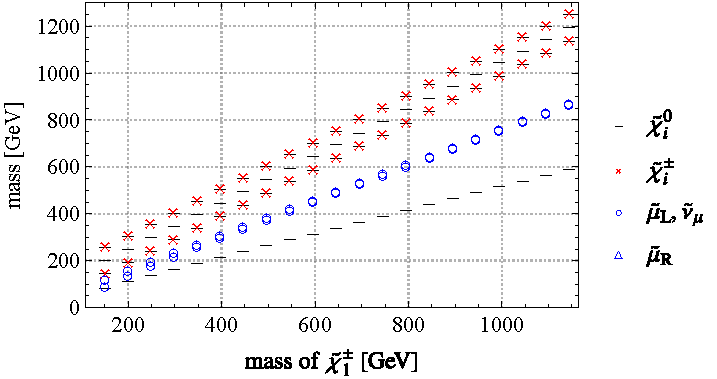
\includegraphics[height=125pt]{../plots/plot_data_tab1_x050.pdf}
  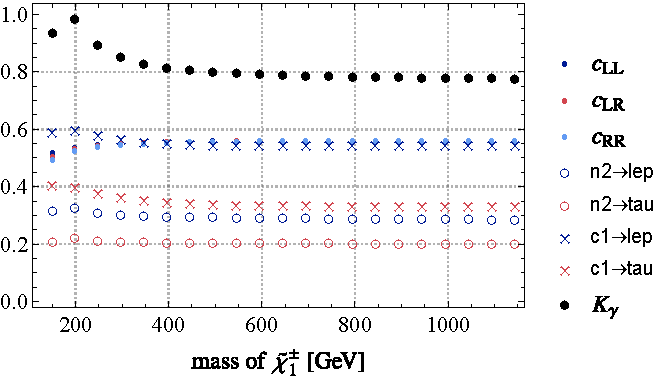
\includegraphics[height=125pt]{../plots/plot_data_tab1_x050_cfactors.pdf}
  \caption{Mass spectrum etc.\ of tab1-0.50 benchmark line. The models are generated with $M_2=200,250,\dots,1200\GeV$, while $m_{\charPM[1]}$ is used as labels.}
\end{figure}

This line is characterized by
\begin{equation}
 M_2=\mu=2M_1,
\quad
 x = \frac{m_{\tilde l\w L}-m_{\neut[1]}}{m_{\neut[2]}-m_{\neut[1]}}=0.5,
\quad
 \tan\beta=40,
\quad
 \tilde l\w R, \tilde q, \text{heavy-Higgs: decoupled}.
\end{equation}
The mass spectrum is shown in the figure; we use $m_{\charPM[1]}$ to label each model point.

Points with $m_{\charPM[1]}<300\GeV$ is not considered in our analysis, since neither by ATLAS.
For $m_{\charPM[1]}>300\GeV$, the LSP is $\neut[1]$ and $\neut[2,3,4]\charPM[1,2]$ may give NC/3L-chain.
We safely ignore $\neut[3]$ because of non-degeneracy and smaller production rate, as it has less $\tilde W$-component.
A degenerate pair $\neut[4]\charPM[2]$ may serve as the chain-3L target, but since we have no way to include its contribution, we ignore it, which has a smaller production rate.
Hence, we consider only the NC/3L chain produced by $pp\to\neut[2]\charPM[1]$.

The cross section is, since the $c$-factors are similar for $m_{\charPM[1]}>300\GeV$, given by
\begin{equation}
 \sigma(pp\to\neut[2]\charPM[1])\approx K_{\sigma}\cdot \sigma(pp\to\tilde W^\pm\tilde W^3);
\qquad
 K_\sigma = \mathop{\mathrm{mean}}(c\w{LL},c\w{LR},c\w{RR}),
\end{equation}
where the pure-wino production cross section $\sigma(pp\to\tilde W^\pm\tilde W^3)$ is taken from LHCSUSYXSWG\footnote{\url{https://twiki.cern.ch/twiki/bin/view/LHCPhysics/SUSYCrossSections13TeVn2x1wino}}.
The cross section is then compared with
\begin{equation}
 \frac{A\w{original}}{A_X}\sigma\w{UL;original}=\frac{1}{K_\Gamma}\sigma\w{UL;original}.
\end{equation}

The results against ATLAS1803 is shown in \cref{fig:tab1_x050_atlas1803}, where the black dots correspond to $K_\sigma K_\Gamma \sigma(\text{Wino})$.
It shows that the ATLAS1803 analysis nearly excludes below $\sim860\GeV$.
The wiggles in $\sigma\w{UL}$ is due to interpolation of the $\sigma\w{UL}$-grid ATLAS provides, for which logarithmic interpolation (i.e., linear interpolation on the function $\log\sigma\w{UL}(m_{\charPM[1]},m_{\neut[1]})$) is used.



\bibliography{analysis}
\end{document}
